
\begin {tikzpicture}[-latex ,auto ,node distance =1 cm,
state/.style ={ circle,draw,minimum width =1 cm}]

\node[state] (A) [] {$s_1$};
\node[state] (B) [above right=of A] {$s_2$};
\node[state] (C) [right=of B] {$s_3$};
\node[state] (D) [below right=of C] {$s_4$};
\node[state] (E) [ below left=of D] {$s_5$};
\node[state] (F) [left=of E] {$s_6$};
\node (01) [left =of A] {$$};

\path (01) edge [dashed] node[above =0.15 cm] {$10$} (A);
\path (A) edge [bend left =25] node[above =0.15 cm] {$4$} (B);
\path (B) edge [bend left =25] node[above =0.15 cm] {$-2$} (C);
\path (C) edge [bend left =25] node[above =0.15 cm] {$3$} (D);
\path (D) edge [bend left =25] node[below =0.15 cm] {$-2$} (E);
\path (E) edge [bend left =25] node[below =0.15 cm] {$-5$} (F);
\path (F) edge [bend left =25] node[below =0.15 cm] {$1$} (A);
\end{tikzpicture}
\hskip 2cm 
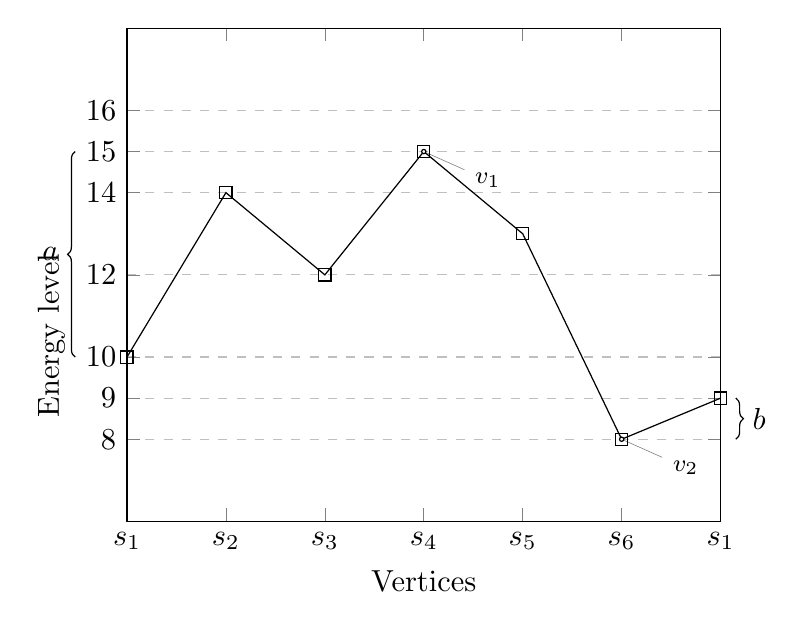
\begin{tikzpicture}[scale=1.1]
\begin{axis}[
    title={},
    xlabel={Vertices},
    ylabel style= {xshift=-20pt},
    ylabel={Energy level},
    clip=false,
    xmin=1, xmax=7,
    ymin=6, ymax=18,
    xtick={1,2,3,4,5,6,7},
    ytick={8,9,10,12,14,15,16},
    xticklabels={$s_1$,$s_2$,$s_3$,$s_4$,$s_5$,$s_6$,$s_1$},
     legend pos=north east,
    ymajorgrids=true,
    grid style=dashed,
]

\addplot[
    color=black,
    mark=square,
    ]
    coordinates {
    (1,10)(2,14)(3,12)(4,15)(5,13)(6,8)(7,9)
    }; 

\node[inner sep=0.5pt,circle,draw,fill=white,pin=-15:\footnotesize $v_1$] 
	  at (axis cs:4,15) {};
	  \node[inner sep=0.5pt,circle,draw,fill=white,pin=-15:\footnotesize $v_2$] 
	  at (axis cs:6,8) {};


\draw[decorate,decoration={brace}]
  ([xshift=-17pt]axis cs:1,10) --
    node[left=2pt] {$a$} 
  ([xshift=-17pt]axis cs:1,15);

\draw[decorate,decoration={brace,mirror}]
  ([xshift=5pt]axis cs:7,8) --
    node[right=2pt] {$b$} 
  ([xshift=5pt]axis cs:7,9);
\end{axis}
\end{tikzpicture}
\caption{Energy level of a negative cycle}
